\chapter{Introducción}
En este capítulo se introducirá el proyecto. Hablaremos sobre el contexto y la motivación por la cual se decidió llevarlo a cabo. Se hará un resumen de los objetivos que se esperaban alcanzar y las soluciones propuestas para alcanzarlos. Y también se llevará a cabo en esta sección un breve resumen de los siguientes apartados de la memoria.

%%%
\section{Motivación}

Estamos en plena revolución digital, durante la cual hemos presenciado un desarrollo increíble de los dispositivos móviles. Desde los primeros que sólo permitían llamar, hasta los que tenemos hoy en día, que nos permiten consultar el correo, subir fotos a las redes sociales, decirnos como llegar a los sitios, etcétera. Pero lo más importante es la difusión que han tenido estos aparatos, en Mayo de 2017 se registraron más de 5.000 millones de líneas activas y no sería de extrañar que en unos años hayan muchas más líneas que personas en el mundo. Debido a su facilidad de uso y a su gran utilidad los sistemas operativos más utilizados son \textit{Android} e \textit{iOS}.

\begin{figure}[t] 
\begin{center}
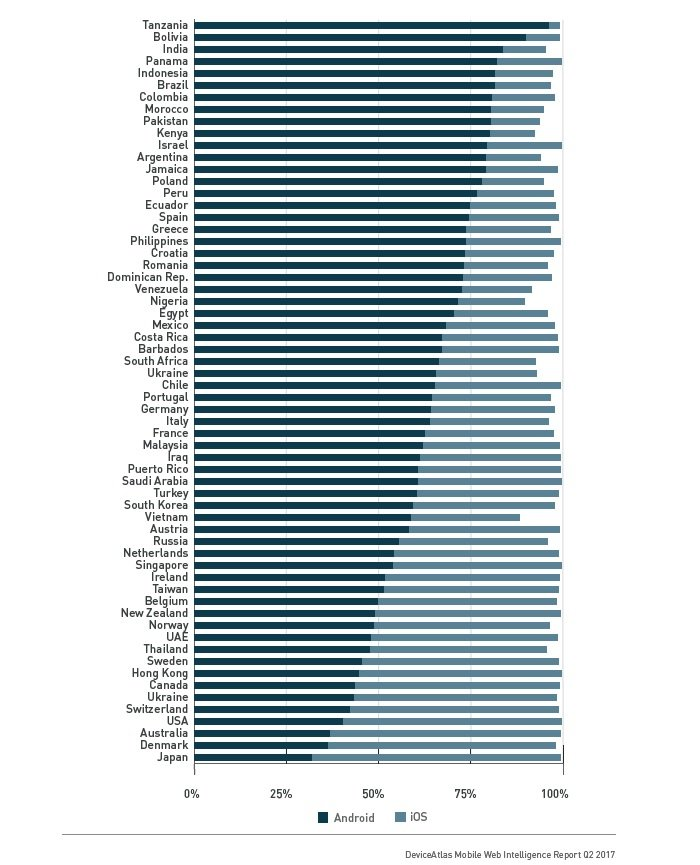
\includegraphics[scale=0.6]{figures/ios_android.jpg}
\caption{\textit{Android} vs \textit{iOS} en diferentes países.\label{fig:and_vs_ios}}
\end{center}
\end{figure}

Como vemos en la figura~\ref{fig:and_vs_ios}, \textit{Android} tiene una mayor aceptación entre el público, sobre todo porque estos móviles tienen precios más asequibles que los que tienen \textit{iOS}. \textit{Android} es utilizado por diversos fabricantes de teléfonos móviles, por esto es que hay mucha competencia y los precios bajan, pero la parte mala de esto es que tenemos un amplio abanico de \textit{Hardware} con diferentes requisitos, complicando la tarea al programador. Los terminales de \textit{Apple} son más caros pero su \textit{Hardware} está especialmente diseñado y optimizado para funcionar de la mano con su propio sistema operativo.

Los terminales móviles poseen una gran cantidad de sensores, entre ellos se encuentra un receptor \textit{GPS}, el cual se puede utilizar para obtener nuestra posición en cualquier punto del globo. Pero esta tecnología tiene un punto débil: los espacios interiores, ya que en ellos la señal no penetra adecuadamente y no puede darnos nuestra ubicación con exactitud. Aquí aparece una nueva necesidad, a la que se ha intentado dar solución en los últimos años de diferentes maneras: con \textit{WiFi}, \textit{Bluetooth}, y otras tecnologías inalámbricas. Pero todavía hay muchas barreras, como la obligación de calibrar el entorno previamente o la necesidad de infraestructura auxiliar como transmisores \textit{Bluetooth} o \textit{WiFi} auxiliares.

En nuestro caso, utilizaremos esta tecnología para la obtención de publicidad basada en la ubicación del cliente dentro de centros comerciales. Y los datos sobre la posición del usuario serán proporcionados por la plataforma \textit{Situm}, que nos da la localización de un usuario en un entorno previamente calibrado con una precisión bastante buena. Gracias a esta aplicación, las tiendas podrán emitir publicidad por un nuevo canal y los consumidores podrán disfrutar de ofertas, descuentos y estar al tanto de productos de su interés que se encuentren en su entorno.


\section{Objetivos}
El objetivo principal de este proyecto es crear una red publicitaria que se distribuirá entre los potenciales clientes según su ubicación en tiempo real. Se utilizarán técnicas de posicionamiento en interiores para solventar las limitaciones de cobertura propias del \textit{GPS}, pero sin dejarlo de lado, de tal manera que la aplicación podrá utilizarse en espacios abiertos y cerrados. Los objetivos principales serán los siguientes:
\begin{itemize}
\item Autenticación de los usuarios y asignación por roles.
\item Publicación de ofertas.
\item Disfrute de dichas ofertas por parte de los clientes.
\end{itemize}

%%
\section{Propuesta}
Proponemos desarrollar una plataforma de publicidad geolocalizada  divida en tres componentes:
\begin{enumerate}
\item \textbf{Sistema de localización de interiores.} Se utilizarán los servicios ofrecidos por la plataforma \textit{Situm}.
\item \textbf{Sistema de almacenamiento en la nube.} Para almacenar toda la información relativa a usuarios, ofertas, tiendas, edificios, roles, permisos e imágenes. Nos hemos decantado por la \textit{API} de \textit{Firebase Google}, que nos ofrece gran cantidad de servicios en la nube, aunque hay otros muchos disponibles. Los servicios de \textit{Firebase} que usaremos en este proyecto serán: base de datos no relacional, \textit{API REST}, \textit{Cloud Functions} y autenticación. 
\item\textbf{ Aplicación móvil \textit{iOS}.} Será la parte de cliente, que se comunicará con los servidores de \textit{Situm} y con \textit{Firebase} a través de su \textit{API REST}. La interfaz y las acciones que podrá llevar a cabo el usuario, dependerán de su rol.
\end{enumerate}

\section{Estructura de la memoria}
En los capítulos siguientes, se profundizará en las múltiples fases del desarrollo de este proyecto. A continuación, un breve resumen del contenido de estos:
\begin{itemize}
\item \textbf{Estado del arte.} Aplicaciones de la localización en interiores en la actualidad.
\item \textbf{Fundamentos teóricos.} Bases teóricas sobre las que se asienta la tecnología de posicionamiento en interiores.
\item \textbf{Fundamentos tecnológicos.} Este capítulo explicará las tecnologías empleadas para el desarrollo de este proyecto en concreto.
\item \textbf{Análisis.} Este capítulo tratará el análisis de requisitos, actores y casos de uso.
\item \textbf{Metodología.} Aquí se explicará la elección de la metodología de desarrollo y su adaptación a este proyecto concreto.
\item \textbf{Gestión de proyecto.} En este capítulo se hablará sobre la planificación de las tareas, estimaciones de costes y valoración de riesgos.
\item \textbf{Arquitectura.} Se expondrá la arquitectura del proyecto, como se estructuraron los diferentes componentes.
\item \textbf{Implementación.} Se tratarán aquí los detalles de la implementación, a partir de la arquitectura comentada en el capítulo anterior.
\item \textbf{Pruebas.} Se hablará sobre las pruebas realizadas a lo largo de la realización del proyecto y al final del mismo.
\item \textbf{Conclusiones.} Como cierre de la memoria, hablaremos sobre las  conclusiones, lecciones aprendidas a lo largo de todo el desarrollo y del trabajo que nos queda por delante en caso de continuar con el proyecto.
\item{}\textbf{Instalación y uso.} En este apéndice, se guiará al usuario a través del proceso de instalación de la aplicación y se le indicará como utilizar las funcionalidades básicas.
\end{itemize}

